\documentclass[11pt]{article}
\usepackage{minted, tikz}
\usepackage{amsfonts, amssymb, amsmath, float, tabularx}
\usepackage{enumerate, esint, nicefrac, algorithm2e}
\parindent 0px
\date{\today}
\title{CS301 :: Final Exam}
\author{Ryan Magdaleno}

% Helpful ::
% \line(1,0){358px}

\begin{document}
\maketitle

%%%%%%%%%%%%%%%%%%%%%%%%%%%%%%%%%%%%%%%%%%%%%%%%%%%%%%%%%%%%%%%%%%%%%%%%%%%%%%%%%%%%%%%%%

\textbf{Problem 1. Multiple Choice.} 

Note: I will only write what I chose, I got this section fully correct.

\vspace{5px}\textbf{Solution ::}
\begin{enumerate}[a.]
    \item Which of the following languages is not in NP? \\ $L=\emptyset$.
    \item T/F. The Turing Recognizable languages are closed under complement. \\ False.
    \item Which of the following languages is undecidable? \\ $EQ_{CFG}$.
    \item Context-Free Languages are closed under which of the following \\
    operations:\\Kleene star.
    \item T/F. All binary languages are Turing-Recognizable.\\ False.
    \item Which of the following is not a constrain of the pumping lemma for
    context-free languages? \\ $|y|\ge 1$.
    \item If we have DFAs $M_1$ with $|Q_1|$ states and $M_2$ with $|Q_2|$ states,
    how many states are in the DFA which decides their intersection?
    \\$|Q_1|\cdot |Q_2|$.
    \item All languages in $P$ must be at most as complex as which of the following?\\
    Turing Decidable Languages.
    \item Which of the following is the definition of the transition function for 
    \\NFAs?\\
    $Q \times (\Sigma\cup\epsilon)\rightarrow P(Q)$.
    \item What is the definition of a Turing Decidable language? \\
    There exists a TM which accepts all strings in the language and rejects all
    strings not in the language.
\end{enumerate}
\pagebreak

%%%%%%%%%%%%%%%%%%%%%%%%%%%%%%%%%%%%%%%%%%%%%%%%%%%%%%%%%%%%%%%%%%%%%%%%%%%%%%%%%%%%%%%%%

\textbf{Problem 2. Short Answer}
\begin{enumerate}[a.]
\item
Give an example of a language that is not finite and not Context-Free. \\
\vspace{5px}\textbf{Solution ::}
$$L = \{0^n1^n0^n \,|\, n\ge 0\}$$
\line(1,0){344px}

\item 
What does it mean for a language to be in NP? \\
\vspace{5px}\textbf{Solution ::} \\
It means that, that language has some TM that can solve it in a \\nondeterministic
manner and can be verified in a polynomial time \\complexity like $O(n)$ for example.
The time to solve it may be exponential or higher.

Also NP may be $==$ P but unknown for now. \\
\line(1,0){344px}

\item
Provide the 5-tuple for the following DFA.
\begin{center}
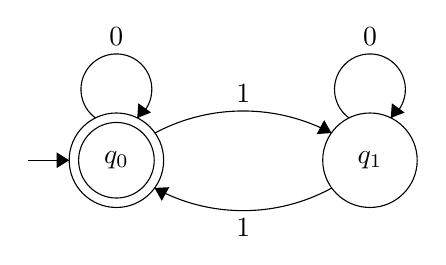
\begin{tikzpicture}[scale=0.2]
\tikzstyle{every node}+=[inner sep=0pt]
\draw [black] (22.2,-31.1) circle (3);
\draw (22.2,-31.1) node {$q_0$};
\draw [black] (22.2,-31.1) circle (2.4);
\draw [black] (38.3,-31.1) circle (3);
\draw (38.3,-31.1) node {$q_1$};
\draw [black] (24.643,-29.372) arc (118.05913:61.94087:11.92);
\fill [black] (35.86,-29.37) -- (35.39,-28.55) -- (34.92,-29.44);
\draw (30.25,-27.47) node [above] {$1$};
\draw [black] (35.881,-32.861) arc (-61.28276:-118.71724:11.72);
\fill [black] (24.62,-32.86) -- (25.08,-33.68) -- (25.56,-32.81);
\draw (30.25,-34.8) node [below] {$1$};
\draw [black] (16.6,-31.1) -- (19.2,-31.1);
\fill [black] (19.2,-31.1) -- (18.4,-30.6) -- (18.4,-31.6);
\draw [black] (20.877,-28.42) arc (234:-54:2.25);
\draw (22.2,-23.85) node [above] {$0$};
\fill [black] (23.52,-28.42) -- (24.4,-28.07) -- (23.59,-27.48);
\draw [black] (36.977,-28.42) arc (234:-54:2.25);
\draw (38.3,-23.85) node [above] {$0$};
\fill [black] (39.62,-28.42) -- (40.5,-28.07) -- (39.69,-27.48);
\end{tikzpicture}
\end{center}
\vspace{5px}\textbf{Solution ::}
\begin{align*}
    Q &= \{q_0, q_1\} \\
    \Sigma &= \{0,1\} \\
    q_0 &= q_0 \\
    F &= \{q_0\} \\
    \delta &= 
    \begin{tabularx}{0.3\textwidth} { 
        | >{\centering\arraybackslash}X 
        | >{\centering\arraybackslash}X 
        | >{\centering\arraybackslash}X | }
        \hline & 0 & 1 \\
        \hline $q_0$ & $q_0$  & $q_1$  \\
        \hline $q_1$ & $q_1$  & $q_0$  \\
        \hline
    \end{tabularx}
\end{align*}
\pagebreak

\item What are the elements of the 7-tuple for a Turing Machine? \\
\vspace{5px}\textbf{Solution ::}
\begin{align*}
    Q &= \text{Set of states.} \\
    \Sigma &= \text{Input alphabet.} \\
    \Gamma &= \text{Tape alphabet.} \\
    \delta &= \text{Transition function: } \\
    &\hspace{16px}Q'\times\Gamma
    \rightarrow Q\times\Gamma\times\{L, R\} \\
    &\hspace{16px}Q' = Q - \{q_{accept}, q_{reject}\} \\
    q_0 &= \text{Start state.} \\
    q_{accept} &= \text{Accept state.} \\
    q_{reject} &= \text{Reject state.} \\
    &\hspace{16px}q_0\in Q \\
    &\hspace{16px}q_{accept}\in Q \\
    &\hspace{16px}q_{reject}\in Q
\end{align*}
\line(1,0){344px}

\item What is the definition of a regular language? \\
\vspace{5px}\textbf{Solution ::} \\
There exists a DFA which can generate that regular language.
\end{enumerate}
\pagebreak

%%%%%%%%%%%%%%%%%%%%%%%%%%%%%%%%%%%%%%%%%%%%%%%%%%%%%%%%%%%%%%%%%%%%%%%%%%%%%%%%%%%%%%%%%

\textbf{Problem 3. NFA Construction} \\
Give an NFA which decides the following language $L$. $\Sigma=\{0,1\}$.
$$L = (11\cup00)^*(00^*\cup 1)$$

\vspace{5px}\textbf{Solution ::}
\begin{center}
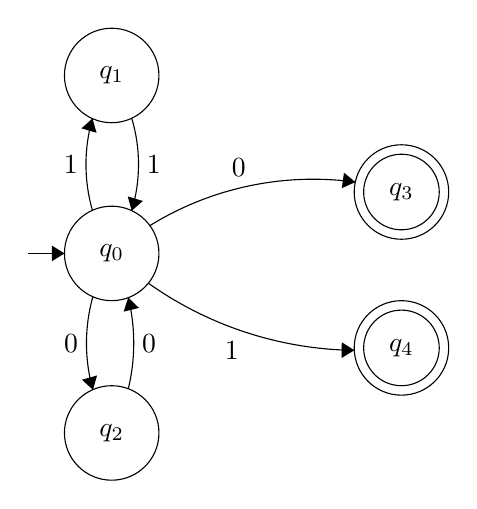
\begin{tikzpicture}[scale=0.2]
\tikzstyle{every node}+=[inner sep=0pt]
\draw [black] (14.3,-27.7) circle (3);
\draw (14.3,-27.7) node {$q_0$};
\draw [black] (14.3,-16.4) circle (3);
\draw (14.3,-16.4) node {$q_1$};
\draw [black] (14.3,-39.1) circle (3);
\draw (14.3,-39.1) node {$q_2$};
\draw [black] (32.7,-23.8) circle (3);
\draw (32.7,-23.8) node {$q_3$};
\draw [black] (32.7,-23.8) circle (2.4);
\draw [black] (32.7,-33.7) circle (3);
\draw (32.7,-33.7) node {$q_4$};
\draw [black] (32.7,-33.7) circle (2.4);
\draw [black] (9,-27.7) -- (11.3,-27.7);
\fill [black] (11.3,-27.7) -- (10.5,-27.2) -- (10.5,-28.2);
\draw [black] (13.077,-24.972) arc (-163.97641:-196.02359:10.584);
\fill [black] (13.08,-19.13) -- (12.38,-19.76) -- (13.34,-20.04);
\draw (12.17,-22.05) node [left] {$1$};
\draw [black] (15.57,-19.106) arc (16.73562:-16.73562:10.224);
\fill [black] (15.57,-24.99) -- (16.28,-24.37) -- (15.32,-24.08);
\draw (16.5,-22.05) node [right] {$1$};
\draw [black] (13.105,-36.359) arc (-164.30611:-195.69389:10.937);
\fill [black] (13.11,-36.36) -- (13.37,-35.45) -- (12.41,-35.72);
\draw (12.2,-33.4) node [left] {$0$};
\draw [black] (15.354,-30.501) arc (13.62845:-13.62845:12.304);
\fill [black] (15.35,-30.5) -- (15.06,-31.4) -- (16.03,-31.16);
\draw (16.2,-33.4) node [right] {$0$};
\draw [black] (16.722,-25.935) arc (121.72964:82.20456:19.723);
\fill [black] (29.77,-23.17) -- (29.05,-22.57) -- (28.91,-23.56);
\draw (22.37,-22.83) node [above] {$0$};
\draw [black] (29.706,-33.855) arc (-90.75539:-125.36555:23.124);
\fill [black] (29.71,-33.85) -- (28.91,-33.34) -- (28.9,-34.34);
\draw (21.92,-33.26) node [below] {$1$};
\end{tikzpicture}
\end{center}
\pagebreak

%%%%%%%%%%%%%%%%%%%%%%%%%%%%%%%%%%%%%%%%%%%%%%%%%%%%%%%%%%%%%%%%%%%%%%%%%%%%%%%%%%%%%%%%%

\textbf{Problem 4. CFG Construction} \\
Give a CFG which generates the following language $L$. $\Sigma = \{a, b\}$.
$$L = \{(a^ib^{2i}b^ja^j)^* \,|\, i\ge 1, j\ge 0\}$$
\vspace{5px}\textbf{Solution ::}
\begin{align}
    S &\longrightarrow AZS \,|\,\epsilon \\
    A &\longrightarrow aBbb \\
    B &\longrightarrow\epsilon\,|\,aBbb \\
    Z &\longrightarrow\epsilon\,|\,bZa
\end{align}
\pagebreak

%%%%%%%%%%%%%%%%%%%%%%%%%%%%%%%%%%%%%%%%%%%%%%%%%%%%%%%%%%%%%%%%%%%%%%%%%%%%%%%%%%%%%%%%%

\textbf{Problem 5. Non-Regular Language} \\
Prove that the following language $L$ is not regular.
$$L = \{w\in\{0,1\}^*\,|\,
\text{ the number of 0's is at least twice the number of 1's}\}.$$
\vspace{5px}\textbf{Solution ::} \\
Let's assume $L$ is regular for the sake of contradiction. There must be some DFA
that decides it. Therefore there must be a pumping length $p$. \\
Let $s = 1^p0^{2p}$, $s\in L$.

$s$ can be partitioned into $xy^iz$, $i\ge 0$. \\
$x$ must be some $1^\alpha$ number of 1s, $0\le\alpha\le p-\beta$. \\
$y$ must be some $i\beta$ number of 1s, $1\le\beta\le p-\alpha$, $i\ge 0$. \\
$z$ must be the remaining 1s and 0s from s. \\
$xy$ are within $p$, $\alpha+\beta\le p$. If we pick $i=2$ for $y$ we get the
following:
$$1^\beta 1^{2\beta} 1^{p-\alpha -\beta}0^{2p}\longrightarrow 1^{\beta+ p}0^{2p}$$
However, we get the contradiction $2(p+\beta)$ 1s not being $==$ to the $2p$ 0s,
because $\beta$ will always be atleast 1.

$\therefore L$ is not regular. 
\pagebreak

%%%%%%%%%%%%%%%%%%%%%%%%%%%%%%%%%%%%%%%%%%%%%%%%%%%%%%%%%%%%%%%%%%%%%%%%%%%%%%%%%%%%%%%%%

\textbf{Problem 6. Turing Decidability} \\
Give an implementation-level description for a Turing Machine $M$ which decides
the following language $L$. You must include an argument that $M$ halts.
$$L = \{0^i1^j2^j\,|\, j\ge 0, i>j\},\,\,\Sigma =\{0,1,2\}$$
\vspace{5px}\textbf{Solution ::}

$M =$ "On input string $w$,
\begin{enumerate}[\hspace{20px}1.]
\item
Check that $w$ is of form $0^*1^*2^*$.

\item
Scan right until an unmarked 0 is found if none are found then reject,
else mark 0.

\item Scan right until an unmarked 1 is found, if found mark it and go to
step 5 else go to step 4.

\item 
Scan right until an unmarked 2 is found, if found then reject, else go to
step 8.

\item 
Scan right until an unmarked 2 is found, mark it, if not found, reject.

\item 
Return head to front of tape.

\item
Go to step 2.

\item
Return head to front of tape and unmark rightmost 0.

\item Scan right and check if there are no unmarked 0s, reject is so. Check
then that no 1 or 2 were left unmarked if so reject, else accept."
\end{enumerate}

\textbf{Halting Justification ::} \\
This will halt because the TM will eventually mark all characters which will
then enter an accept or reject state.
\pagebreak

%%%%%%%%%%%%%%%%%%%%%%%%%%%%%%%%%%%%%%%%%%%%%%%%%%%%%%%%%%%%%%%%%%%%%%%%%%%%%%%%%%%%%%%%%

\textbf{Problem 7. Undecidability Proof} \\
Prove that the following language is undecidable via reduction.
$$THREE_{TM} = \{\langle M\rangle\,|\, M
\text{is a TM that accepts exactly 3 strings}\}$$
\vspace{5px}\textbf{Solution ::} \\
Suppose for the sake of contradiction that $THREE_{TM}$ is decidable, therefore
a TM $Z$ decides it. Define the following TM $A$:

\vspace{5px}$A$ = "On input $\langle M, w\rangle$,

\hspace{30px}$M'=$ "On input $x$,

\hspace{45px}If $x\notin\{0,1,01\}$, reject.

\hspace{45px}Return $M(w)$.

\hspace{30px}Simulate $Z$ with $\langle M'\rangle$, if $M'$ accepts, then $Z$
accepts, else $Z$ rejects.

\vspace{5px}$A$ accepts exactly when $M$ accepts $w$, and rejects otherwise.
This is a contradiction since we know $A_{TM}$ is undecidable.

$\therefore THREE_{TM}$ is undecidable.

\pagebreak

\end{document}